\chapter{导数的应用}
\section{用导数研究函数的例子}
\subsection{三次函数}


\begin{example}
    \(a > 0\)，函数 \(f(x) = x^4 + x^3 + ax + a^2\) 有且仅有两个不同的零点，求\(a\) 的取值范围。
\end{example}
\begin{jie}
    \


    \begin{way1}
        求导得\(f'(x)=4x^3+3x^2+a\). 常数项\(a\)可以看做对函数\(g(x)=4x^3+3x^2\)的平移. 因式分解得
        \(g(x)=x^2(4x+3)\), 由此绘制出图像
        \begin{figure}[H]

              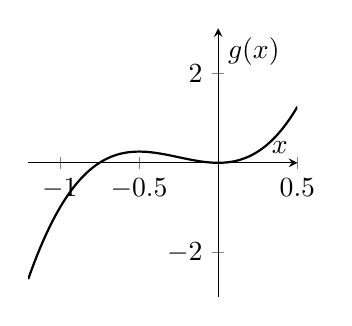
\begin{tikzpicture}
                \begin{axis}[
                    axis lines = middle, % 设置坐标轴为中间形式
                    xlabel = {$x$},     % x轴标签
                    ylabel = {$g(x)$},     % y轴标签
                    ymin = -3, ymax = 3, % y轴范围
                    xmin = -1.2, xmax = 0.5, % x轴范围
                    domain = -1.2:0.5,    % 函数的定义域
                    samples = 100,      % 采样点数量
                    width=5cm, height=5cm % 图像大小
                ]
                % 绘制函数图像
                \addplot [thick] {4*x^3 + 3*x^2};
                \end{axis}
               \end{tikzpicture}  
              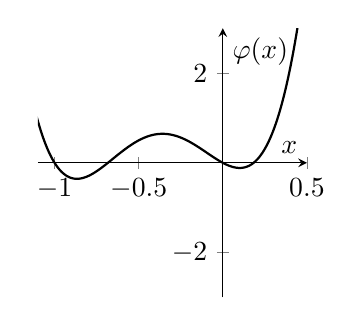
\begin{tikzpicture}
                \begin{axis}[
                    axis lines = middle, % 设置坐标轴为中间形式
                    xlabel = {$x$},     % x轴标签
                    ylabel = {$\varphi(x)$},     % y轴标签
                    ymin = -3, ymax = 3, % y轴范围
                    xmin = -1.1, xmax = 0.5, % x轴范围
                    domain = -1.2:0.5,    % 函数的定义域
                    samples = 1000,      % 采样点数量
                    width=5cm, height=5cm % 图像大小
                ]
                % 绘制函数图像
                \addplot [thick] {16*x^4 + 24*x^3+6*x^2-2*x^1};
                \end{axis}

            \end{tikzpicture}
            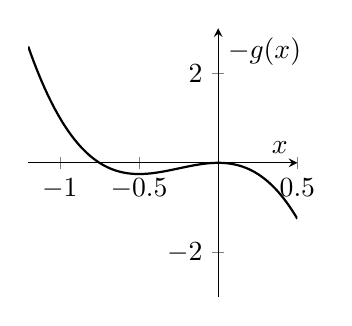
\begin{tikzpicture}
                \begin{axis}[
                    axis lines = middle, % 设置坐标轴为中间形式
                    xlabel = {$x$},     % x轴标签
                    ylabel = {$-g(x)$},     % y轴标签
                    ymin = -3, ymax = 3, % y轴范围
                    xmin = -1.2, xmax = 0.5, % x轴范围
                    domain = -1.2:0.5,    % 函数的定义域
                    samples = 100,      % 采样点数量
                    width=5cm, height=5cm % 图像大小
                ]
                % 绘制函数图像
                \addplot [thick] {-4*x^3 - 3*x^2};
                \end{axis}
               \end{tikzpicture}  
        \end{figure}
        由于\(a>0\), 从\(g(x)\)图像可见向上平移中不会为\(f'(x)\)增加更多零点了。即\(f'(x)\)在\(\mathbb{R}\)上有唯一的
        变号零点\(x_0\), 满足
        \begin{equation}
            4x_0^3+3x_0^2+a=0. 
        \end{equation}
        \(f(x)\)在\((-\infty,x_0)\)单调递减, 在\((x_0,+\infty)\)单调递增.因此只要\(f(x_0)<0\), 即可满足
        \(f(x)\)在\((-\infty,x_0)\)和\((x_0,+\infty)\)分别有唯一零点.

        在消去\(x_0\)和消去\(a\)的选择中, 这里选择了消\(a\), 带入\(a=-(4x_0^3+3x_0^2) \)
        \begin{align*}
            f(x)&=x^4_0+x^3_0+ax_0+a^2\\
                &=x^4_0+x^3_0+x_0(-4x_0^3-3x_0^2)+(-4x_0^3-3x_0^2)^2\\
                &=16x_0^6+24x_0^5+6x_0^4-2x_0^3\\
                &=2x_0^3(8x_0^3+12x_0^2+3x_0-1)\\
                &=2x_0^3(x_0+1)(8x_0^2+4x_0-1)
        \end{align*}
        设\(\varphi(x)=2x^3(x+1)(8x^2+4x-1)\), 其零点为\(-1,\frac{-1-\sqrt{3}}{4},0,\frac{-1+\sqrt{3}}{4}\).绘制出图像如所示,
        故使得\(f(x_0)<0\)的\(x_0\)取值范围是\((-1,\frac{-1-\sqrt{3}}{4})\cup(0,\frac{-1+\sqrt{3}}{4})\).
        
        别忘了\(x_0\)和\(a\)的关系\(-4x_0^3-3x_0^2=a\),我们需要把\(g(x)\)翻折一下. 由于\(a\)必须是正的,且\(\frac{-1-\sqrt{3}}{4}>-\frac{3}{4}\),
        在这个范围内,\(a\)的取值范围是\((0,1)\).
    \end{way1}
    \begin{way2}
        
    \end{way2}
\end{jie}

\clearpage
\subsection{三角函数}
\begin{example}
    已知$x^2+y^2=1$, 求$(2x+2)(5y+9)$的最大值.
\end{example}
\begin{jie}
    \begin{way1}[三角换元]
        做换元\(x=\cos\theta,y=\sin\theta\).
        这原式化为
        \[(2x+2)(5y+9)=10\cos\theta\sin\theta+10\sin\theta+18\cos\theta+18\]
        记\(f(\theta)=5\sin\theta+9\cos\theta+5\sin\theta\cos\theta\),求导得  
        \[f'(\theta)=5\cos\theta-9\sin\theta+5\cos2\theta=0\]
        也即
        \begin{align*}
            5\cos\theta+5\cos2\theta&=9\sin\theta\\
            25(\cos\theta+2\cos^2\theta-1)^2&=81(1-\cos^2\theta)
        \end{align*}
        整理, 记\(\cos\theta=m\),得
        \[100m^4+100m^3+6m^2-50m-56=0\]
        注意到\(m=-1\)是一个根, 因此原式可以分解为
        \[100m^4+100m^3+6m^2-50m-56=2(m+1)(50m^3+3m-28)=0\]
        三次方程\(50m^3+3m-28=0\)唯一一个实根是\(m=\frac{4}{5}\).\qed
    \end{way1}
    \begin{way2}
        考虑Lagrange乘数法,记\(L(x,y,\lambda)=(2x+2)(5y+9)-\lambda(x^2+y^2-1)\).
        计算偏导数
        \[\left\{
            \begin{aligned}
                \frac{\partial L}{\partial x}&=2(5y+9)-2\lambda x=0\\
                 \frac{\partial L}{\partial y}&=5(2x+2)-2\lambda y=0\\
                  \frac{\partial L}{\partial \lambda}&=-(x^2+y^2-1)=0
            \end{aligned}
        \right.\]
        消去\(\lambda\)得到方程组
        \[\left\{
            \begin{aligned}
                &\frac{5y+9}{x}=\frac{5x+5}{y}\\
                &x^2+y^2=1
            \end{aligned}
        \right.\]
        接下来使用三角换元, 和上面得到的方程完全一致.\qed
    \end{way2}
\end{jie}

\begin{theorem}[Fejér-Jackson不等式]
    \(x\in (0,\pi)\), 则有
    \begin{equation}\label{equ:Fejér-Jackson不等式}
        \sum_{k=1}^{n}\frac{\sin kx}{k}>0.
    \end{equation}
\end{theorem}
\begin{proof}
    记\(f_n(x)=\sum_{k=1}^{n}\frac{\sin kx}{k}\), 则求导得
    \begin{align*}
        f'_n(x)&=\sum_{k=1}^{n}\cos kx=\frac{\cos\frac{(n+1)x}{2}\sin\frac{nx}{2}}{\sin\frac{x}{2}}
    \end{align*}
    \(f'n(x)\)的所有零点应该满足
    \[\cos\frac{(n+1)x}{2}=0\text{或}\sin\frac{nx}{2}=0,\]
    也即
    \[\frac{(n+1)x}{2}=\frac{\pi}{2}+k\pi\text{或}\frac{nx}{2}=k\pi\quad(k\in\mathbb{Z}),\]








\end{proof}








\clearpage
\subsection{常见的函数不等式}
\begin{theorem}
    当 $x \geqslant 1$ 时，有 $\ln x \leqslant \frac{1}{2}\left(x - \frac{1}{x}\right)$；当 $0 < x \leqslant 1$ 时，有 $\ln x \geqslant \frac{1}{2}\left(x - \frac{1}{x}\right)$。当且仅当 $x = 1$ 时取等。
\end{theorem}
\begin{proof}
    考虑函数 $\varphi(x) = \ln x - \frac{1}{2}\left(x - \frac{1}{x}\right)$，其中 $x > 0$，计算得 $\varphi(1) = 0$，并且
\[
\varphi'(x) = \frac{1}{x} - \frac{1}{2} - \frac{1}{2x^2} = -\frac{(x-1)^2}{2x^2} \leqslant 0,
\]
从而可知 $\varphi(x)$ 在 $(0, +\infty)$ 内单调递减。因此，当 $x \geqslant 1$ 时，有 $\ln x \leqslant \frac{1}{2}\left(x - \frac{1}{x}\right)$；当 $0 < x \leqslant 1$ 时，有 $\ln x \geqslant \frac{1}{2}\left(x - \frac{1}{x}\right)$。
\end{proof}
\begin{theorem}
    当 $x \geqslant 1$ 时，有 $\ln x \geqslant \frac{2(x-1)}{x+1}$；当 $0 < x \leqslant 1$ 时，有 $\ln x \leqslant \frac{2(x-1)}{x+1}$。当且仅当 $x = 1$ 时取等。
\end{theorem}

\begin{proof}
    考虑函数 $\varphi(x) = \ln x - \frac{2(x-1)}{x+1}$，其中 $x > 0$，计算得 $\varphi(1) = 0$，并且
\[
\varphi'(x) = \frac{1}{x} - \frac{4}{(x+1)^2} = \frac{(x-1)^2}{x(x+1)^2} > 0,
\]
从而可知 $\varphi(x)$ 在 $(0, +\infty)$ 内单调递增。因此，当 $x \geqslant 1$ 时，有 $\ln x \geqslant \frac{2(x-1)}{x+1}$；当 $0 < x \leqslant 1$ 时，有 $\ln x \leqslant \frac{2(x-1)}{x+1}$。
\end{proof}

\tbox{
\[  \frac{2(x-1)}{x+1} \leqslant \ln x \leqslant \frac{1}{2}\left(x - \frac{1}{x}\right); (x\leq 1)\]
\[ \frac{1}{2}\left(x - \frac{1}{x}\right) \leqslant \ln x \leqslant \frac{2(x-1)}{x+1}.(0 < x \leqslant 1)\]

}
\begin{theorem}[对数均值不等式]\label{thm:对数均值不等式}\index{不等式!对数均值不等式}
    设 $a$ 和 $b$ 是互异正数，则
\[
\sqrt{ab} < \frac{a-b}{\ln a - \ln b} < \frac{a+b}{2}.
\]
\end{theorem}
\begin{proof}
    不妨设 $a > b$。对于右边的不等式，整理得
\[
\ln a - \ln b = \ln \frac{a}{b} > \frac{2(a-b)}{a+b} = \frac{2\left(\frac{a}{b} - 1\right)}{\frac{a}{b} + 1},
\]
令 $t = \frac{a}{b} > 1$，则该不等式等价于 $\ln t > \frac{2(t-1)}{t+1}$，这是已经证明的结论。对于左边的不等式，整理得
\[
\ln a - \ln b = \ln \frac{a}{b} < \frac{a-b}{\sqrt{ab}} = \sqrt{\frac{a}{b}} - \sqrt{\frac{b}{a}},
\]
该不等式等价于 $\ln t < \sqrt{t} - \frac{1}{\sqrt{t}}$，这也是已经证明的结论。
\end{proof}

\clearpage
